\begin{frame}
  \titlepage
\end{frame}


\begin{frame}[fragile]
\frametitle{Trie}
\begin{columns}
\begin{column}{0.6\textwidth}
\begin{block}{Trie}
\begin{itemize}
\item
Albero
\item
Query: parola $\in$ dizionario
\item
archi etichettati
\item
Percorso radice-foglia = parola
\end{itemize}
\end{block}
\begin{block}{Dizionario}
ABRACADABRA\\
ARRAY\\
\uncover<3->{\alert{ABRA}}
\end{block}
\end{column}
\begin{column}{0.4\textwidth}
\begin{center}
\onslide<2->{\includegraphics[width=0.5\textwidth]{figures/trie1}}
%\onslide<4->{\includegraphics[width=\textwidth]{figures/trie3}}
\end{center}
\end{column}
\end{columns}
\end{frame}

\begin{frame}[fragile]
\frametitle{Trie}
\begin{columns}
\begin{column}{0.6\textwidth}
\begin{block}{Terminatore}
\$ non appartiene all'alfabeto
\end{block}
\onslide<2->{\begin{block}{Dizionario}
ABRACADABRA\$\\
ARRAY\$\\
ABRA\$
\end{block}}
\end{column}
\begin{column}{0.4\textwidth}
\begin{center}
\onslide<3->{\includegraphics[width=0.8\textwidth]{figures/trie4}}
\end{center}
\end{column}
\end{columns}
\end{frame}

\begin{frame}[fragile]
\frametitle{Suffix tree}
\begin{columns}
\begin{column}{0.5\textwidth}
\begin{block}{Definizione}
\begin{itemize}[<+->]
% \item
% Testo $T$
\item
Trie compatto di tutti i suffissi di $T\$$
\item
Le etichette degli archi uscenti da $x$ iniziano con simboli diversi
\item
suffissi $\Leftrightarrow$ percorso radice-foglia
\end{itemize}
\end{block}
\end{column}
\begin{column}{0.5\textwidth}
\begin{center}
\uncover<4->{\includegraphics[width=\textwidth]{figures/Suffix_tree_BANANA}

BANANA\$}
\end{center}
\end{column}
\end{columns}
\end{frame}

\begin{frame}[fragile]
\frametitle{Suffix tree 2: Definizione}
\begin{itemize}
\item
foglie etichettata con posizione inizio suffisso
\item
path-label$(x)$: concatenazione etichette
\item
string-depth$(x)$: lunghezza path-label$(x)$
\item
Pattern matching = visita
\end{itemize}
\begin{block}{Problemi}
\begin{itemize}[<+->]
\item
Spazio $O(n^{2})$
\item
Puntatori al testo (posizioni)
\item
Spazio $20n$ bytes
\end{itemize}
\end{block}
\end{frame}

\begin{frame}[fragile]
\frametitle{Suffix array}
\begin{block}{Definizione}
\begin{itemize}[<+->]
\item
Array dei suffissi in ordine lessicografico
\item
Posizioni iniziali del suffisso nell'array
\item
Spazio $4n$ bytes
\item
$Lcp[i]$: lunghezza prefisso comune $SA[i]$, $SA[i+1]$
\end{itemize}
\end{block}
\uncover<5->{\begin{block}{BANANA\$}
\begin{tabular}[l]{|c|l|l|l|l|l|l|l|}
\hline
$i$&1&2&3&4&5&6&7\\
$SA$&7&6&4&2&1&5&3\\
$Lcp$&0&1&3&0&0&2&-\\\hline
\end{tabular}}
\end{block}
\end{frame}

\begin{frame}[fragile]
\frametitle{Da Suffix tree a Suffix array}
\begin{columns}
\begin{column}{0.5\textwidth}
\begin{itemize}[<+->]
\item
Visita depth-first di $ST$
\item
archi uscenti di ogni nodo in ordine lessicografico
\item
$Lcp[i]$ = string-depth di $lca(i,i+1)$
\end{itemize}
\end{column}
\begin{column}{0.4\textwidth}
\begin{center}
\onslide<1->{\includegraphics[width=\textwidth]{figures/Suffix_tree_BANANA}}
%\onslide<4->{\includegraphics[width=\textwidth]{figures/trie3}}
\end{center}
\end{column}
\end{columns}
\end{frame}

\begin{frame}[fragile]
\frametitle{Da Suffix array a Suffix tree}
\begin{columns}
\begin{column}{0.5\textwidth}
\begin{itemize}[<+->]
\item
$Lcp = 0$:  partizione $SA$
\item
corrispondono ai figli della radice
\item
ricorsione prendendo i numeri minimi
\end{itemize}
\begin{block}{BANANA\$}
\begin{tabular}[l]{|c|l|l|l|l|l|l|l|}
\hline
$i$&0&1&2&3&4&5&6\\
$SA$&7&6&4&2&1&5&3\\
$Lcp$&0&1&3&0&0&2&-\\\hline
\end{tabular}
\end{block}
\end{column}
\begin{column}{0.5\textwidth}
\begin{center}
\only<2>{\includegraphics[width=\textwidth]{figures/Suffix_tree_BANANA-level1}}
\only<3>{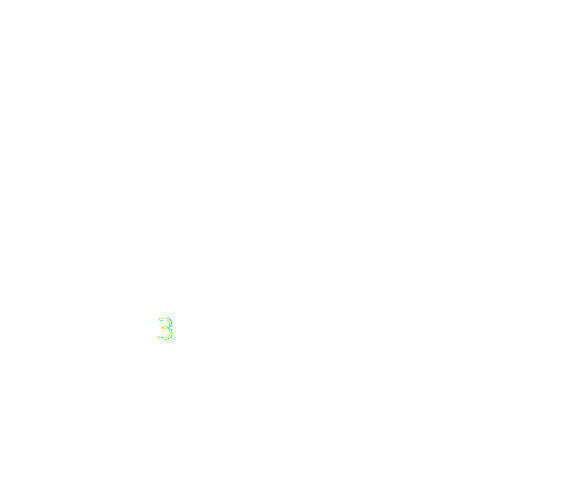
\includegraphics[width=\textwidth]{figures/Suffix_tree_BANANA-level2}}
\only<4>{\includegraphics[width=\textwidth]{figures/Suffix_tree_BANANA-level3}}
\only<5>{\includegraphics[width=\textwidth]{figures/Suffix_tree_BANANA}}
\end{center}
\end{column}
\end{columns}
\end{frame}



\begin{frame}
\frametitle{Suffix tree generalizzato}
\begin{columns}
\begin{column}{0.8\textwidth}
\begin{center}
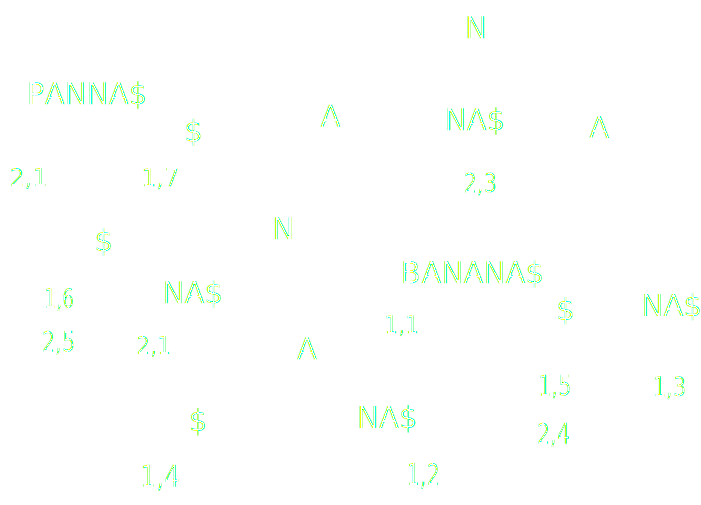
\includegraphics[width=0.8\textwidth]{figures/ST-banana-panna}
\end{center}
\end{column}
\begin{column}{0.18\textwidth}
$s_{1}$: BANANA\$\\
$s_{2}$: PANNA\$
\end{column}
\end{columns}
\end{frame}


\begin{frame}[fragile]
\frametitle{Sottostringa comune più lunga di due stringhe}
\begin{block}{Due stringhe $s_{1}$ e $s_{2}$}
\begin{itemize}[<+->]
\item
Suffix tree generalizzato = insieme di stringhe
\item
$ST(s_{1}\$_{1}s_{2}\$_{2})$
\item
Nodo $x$ con foglie di $s_{1}$ e $s_{2}$
\item
Sottostringa di $s_{1}$ e $s_{2}$
\item
$ST(s_{1}\$s_{2}\$)$
\item
Max string-depth
\end{itemize}
\end{block}
\end{frame}



%%% Local Variables:
%%% TeX-PDF-mode: t
%%% TeX-master: "03-suffix-tree-array-video"
%%% End:
